\chapter{Familiarisation with Inductor}
	\section{Aim}
		\begin{itemize}
			\tightlist
			\item Explain Function of Inductor
			\item Explain the factors influencing inductance
		\end{itemize}
	
	\section{Apparatus}
		\begin{itemize}
			\tightlist
			\item Resistor
			\item Inductor of different forms
			\item 12V Battery
		\end{itemize}	
	
	\section{Theory}
		\subsection{Function of an Inductor}
			\begin{figure}[ht]
				\centering 
				\subfloat[A valve]{
\includegraphics[width=0.3\textwidth,valign=c]{img/exp3/1}
					\label{fig:funcInduc:1}}	
				\hfill
				\subfloat[A resistor]{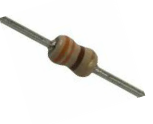
\includegraphics[width=0.3\textwidth,valign=c]{img/exp3/2}
					\label{fig:funcInduc:2}}
				\hfill
				\subfloat[An Inductor]{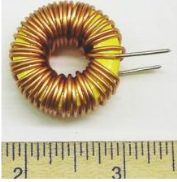
\includegraphics[width=0.3\textwidth,valign=c]{img/exp3/3}
					\label{fig:funcInduc:3}}			
				\caption{\textit{Functioning of an Inductor}}
			\end{figure}
		
			The function of a valve is to control the amount of fluid that flows through a pipe. In an electronic circuit, the resistor is used to control the amount of current that flows through a conductor. Another device that controls the current is the inductor. However unlike the resistor that affects the current uniformly at all times, the inductor only affects currents when thy are changing in value.
		
		\subsection{Similarity with Capacitor}
			\begin{itemize}
				\tightlist
				\item Rate of change of voltage in a capacitor depends upon the current through it. Rate of change of current in an inductor depends upon the voltage applied across it.
				\item Like capacitive current , inductive current is not simply proportional to voltage.
				\item Unlike the situation in a resistor, the power associated with inductive current (V times I) is not turned into heat but is stored as energy in the inductor’s magnetic field.
			\end{itemize}
		
		\subsection{Equation of an Inductor}
			\begin{align*}
				V &= L \frac{dI}{dt}
			\end{align*}
			\begin{itemize}
				\tightlist
				\item $L$ is the inductance and is measured in henry.
				\item Putting a voltage across an inductor causes the current to rise as a ramp.
				\item 1 volt across 1 henry produces a current that increases at 1 amp per second
			\end{itemize}
		
		\subsection{Structure of an Inductor}
			\begin{figure}[ht]
				\centering 
				\subfloat[Structure of different types of Inductors]{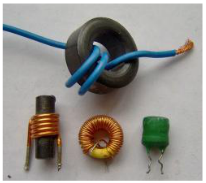
\includegraphics[width=0.45\textwidth,valign=c]{img/exp3/4}
					\label{fig:strInduc}}	
				\hfill
				\subfloat[Internal view of an inductor]{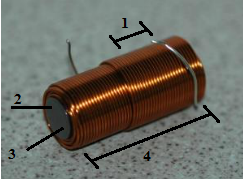
\includegraphics[width=0.45\textwidth,valign=c]{img/exp3/5}
					\label{fig:inductance1}}			
				\caption{\textit{Inductor}}
			\end{figure}
		
			It consists of a wire wound as a coil around a core. The core may consist of a air filled hollow tube or solid material. (See Figure \ref{fig:strInduc})
		
		\subsection{Inductance}
			The amount of inductance in henries a coil has, is determined by the following factors (See Figure \ref{fig:inductance1})-
			\begin{enumerate}
				\tightlist
				\item No of turns of wire wound around the coil
				\item Cross sectional area of the coil
				\item The material type of the coil
				\item The Length of the coil
			\end{enumerate}
		\subsection{Inductive Kick}
			\begin{figure}[h]
				\centering
				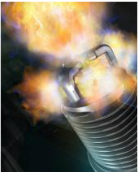
\includegraphics[width=0.5\linewidth]{img/exp3/6}
				\caption{Inductive Kick creating a spark in the spark-plug}
				\label{fig:inductiveKick}
			\end{figure}			
			An Inductive is capable of producing a momentary voltage that is much higher than the voltage of th power source that supplied the current to create its magnetic field . This temporary voltage is called an inductive kick.
			
			Example of applications of inductive devices to provide an inductive kick is a Combustion Engine ignition system that creates the spark across the gap of the spark plug (see Figure \ref{fig:inductiveKick}).

	\section{Conclusion}
		An inductor, also called a coil, choke, or reactor, is a passive two-terminal electrical component that stores energy in a magnetic field when electric current flows through it. An inductor typically consists of an insulated wire wound into a coil. Inductor is an important component of any electronic circuit. Inductance is always present in any circuit, where Inductor is present or not.